\documentclass[aspectratio=169]{beamer}

\usepackage[utf8]{inputenc}

\usepackage{amsfonts}
\usepackage{amsmath}
\usepackage{color}
\usepackage{listings}
\usepackage{tikz}
\usepackage{hyperref}

\newif\ifnotes
  \notesfalse
%  \notestrue

\newif\iftransitions
% \transitionstrue
 \transitionsfalse

\newif\iffast
% \fasttrue
  \fastfalse

\ifnotes
\usepackage{pgfpages}
\setbeameroption{show notes}
\setbeameroption{show notes on second screen=right}
\fi

\usetheme{Rochester}
\usecolortheme{beaver}

\addtobeamertemplate{navigation symbols}{}{%
    \usebeamerfont{footline}%
    \usebeamercolor[fg]{footline}%
    \hspace{1em}%
    \insertframenumber/\inserttotalframenumber
}

\lstloadlanguages{C++}
    \lstset{%
        language={C++},
        basicstyle=\ttfamily,
        keywordstyle=\color{blue},
        showstringspaces=false,
        escapechar={§},
        escapeinside={(*@}{@*)}
    }

\lstdefinestyle{cpp20}{language={C++},
  morekeywords={noexcept,co_await,co_return,co_yield,requires,consteval,constinit,concept}
}

\tikzstyle{every picture}+=[remember picture]

\newcommand{\cpause}{\iftransitions \pause \fi}

\newcommand{\cuncover}[2]{\iftransitions \uncover<#1>{#2} \else #2 \fi}

\definecolor{co_return_object}{RGB}{179,179,255}
\definecolor{co_promise}{RGB}{255,179,179}
\definecolor{co_awaitable}{RGB}{179,255,179}


\title{Safety First!}
\subtitle{Understanding How To Develop Safety-Critical Software}
\author{Andreas Weis}
\institute{Woven by Toyota}

\date{C++Now 2023}
\titlegraphic{
\includegraphics[height=.15\textheight]{resources/cppnow_logo.png}}

\iffalse
Safety-First: Understanding How To Develop Safety-critical Software

Safety-critical software is becoming increasingly visible as a target domain for C++. But what does it actually mean to develop for a safety-critical system? You may have heard wild stories about safety-certified compilers and MISRA conformance checks, but how does that help making software more safe? What does it even mean to be safe? In this talk we will try to shed some lights on the driving factors behind safety-critical development: Gain an understanding of the fundamental principles for reasoning about safety and delve deeply into the implications for day to day software development. We will get you into the mindset of a safety engineer and help you understand both the "how?" and "why?" of common safety engineering practices. Using the ISO standard for functional safety in automotive systems as a starting point, we will illustrate the conceptual models of safety and what the effects of those are on a C++ codebase implementing safety-critical functionalities. In the end, you will hopefully get a better understanding for the needs of developers working in safety-critical domains, and why they sometimes seem at odds with those of ordinary application developers. And how despite the different means being employed, in the end we all are striving for the same goal of writing well-engineered, high quality software. 


Comments:
This talk will be similar in spirit to talks like Michael Wong's CppCon 2019 presentation on safety-critical software, but specifically targeted at the CppNow audience of highly experienced C++ developers with only a vague background in safety. The goal is really to give people a better understanding for the often seemingly strange demands from safety people and help them understand the underlying mindset that drives development in such projects. Especially in light of the increasing attention to concerns from safety people in the ISO C++ committee (eg. P2026), this talk aims to build a bridge of understanding for C++ experts to the safety community. 

Outline:
 * What is Safety? When do we consider software to be "safe". Difference between safe and bug-free.
 * A tour of the ISO-26262 standard. This will mostly be about development processes, but it is an important building block to understand the effects on software development
 * Where safety-critical development differs from ordinary development. And where it doesn't.
 * A critical look at common practices from the safety community and how they relate to the current understanding of best practices in the C++ community
 * A discussion of the fitness of C++ for safety-critical development compared to other languages like C, Ada or Rust
 * Possible future directions for C++ to better support safety use cases
\fi

\begin{document}
{ % all template changes are local to this group.
    \setbeamertemplate{navigation symbols}{}
    \begin{frame}<article:0>[plain]
        \begin{tikzpicture}[remember picture,overlay]
            \node[at=(current page.center)] {
                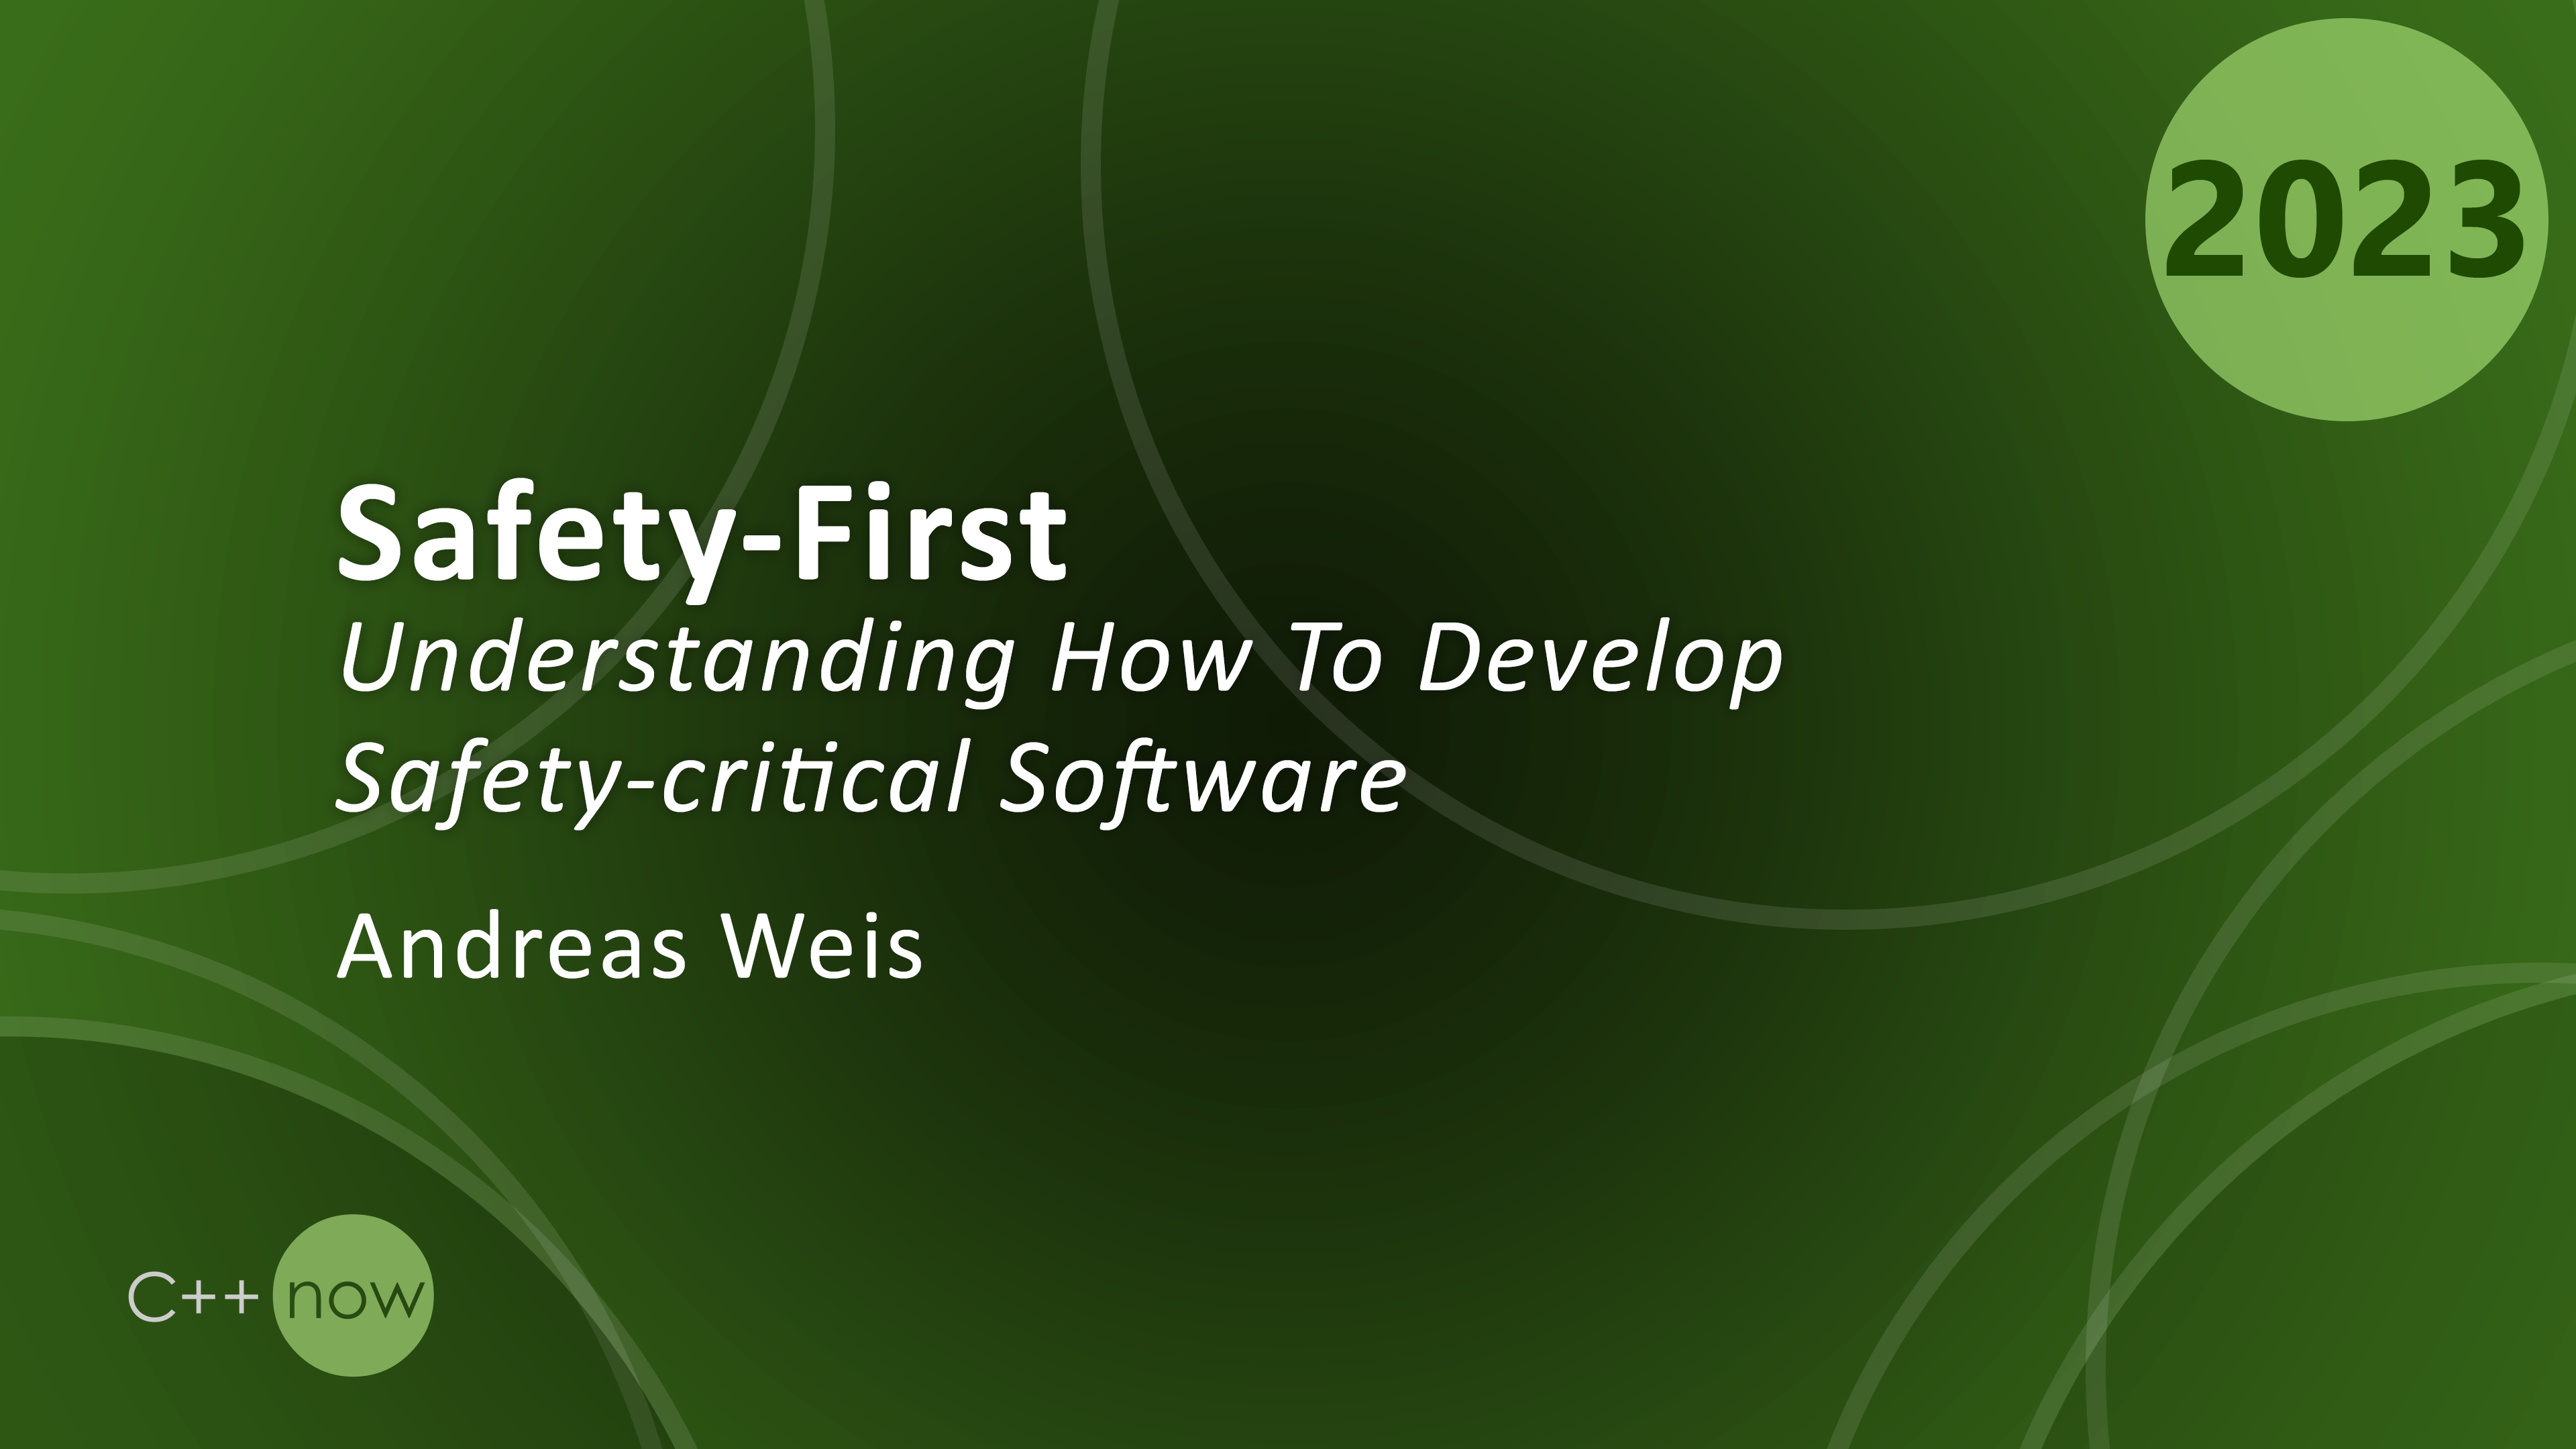
\includegraphics[keepaspectratio,
                                 width=\paperwidth,
                                 height=\paperheight]{safetygfx/title_card.png}
            };
        \end{tikzpicture}
     \end{frame}
}


\frame{\titlepage}

%\iffalse %!!!!!!!!!!!!!!!!!

\begin{frame}[fragile]
  \frametitle{About me - Andreas Weis (he/him)}

  \begin{itemize}
    \setlength\itemsep{1.5em}

    \item \href{https://stackoverflow.com/users/577603/comicsansms}{
\includegraphics[height=.05\textheight]{resources/so-icon.png}} \href{https://github.com/ComicSansMS}{
\includegraphics[height=.05\textheight]{resources/github-icon.png}} \includegraphics[height=.05\textheight]{resources/discord-icon.png} ComicSansMS

    %\item \href{https://twitter.com/DerGhulbus/}{
\includegraphics[height=.05\textheight]{resources/twitter-icon.png} @DerGhulbus}

    \item 
\includegraphics[height=.05\textheight]{resources/meetup-icon.png} Co-organizer of the \href{https://www.meetup.com/MUCplusplus/}{Munich C++ User Group}
    
    \item Working in automotive on safety-critical components since 2017; member of MISRA C++ WG since 2018 member of ISO SC22 WG21 since 2018;

    \item Currently working as a Runtime Engineer for Woven by Toyota \includegraphics[height=.1\textheight]{resources/woven_toyota_logo.png}

  \end{itemize}
\end{frame}

\begin{frame}
  \frametitle{Motivation}
  
  \cpause

  \begin{center}
  
\includegraphics[width=.3\textwidth]{safetygfx/pragmatic_programmer.jpg}
  \hspace{.1\textwidth}
  
\includegraphics[width=.3\textwidth]{safetygfx/software_craftsman.jpg}
  \end{center}

  \note{
  \begin{itemize}
  \item Software Craftsmanship: Programming skills, elegant beautiful programs
  \item Engineering: Responsibility, Methodology, Accountability
  \item When we say safety, we mean regulation
  \item What does it mean to work in a regulated industry?
  \end{itemize}
  }
\end{frame}

\begin{frame}
  \frametitle{Fair Warning}
  
  \begin{center}
  This is going to be a very boring talk.
  \end{center}

\end{frame}

\begin{frame}
  \frametitle{Outline}
  
  \begin{itemize}
    \item What is safety?
    \item What are the regulations around functional safety
    \item A tour of an ISO safety standard for software
    \item Using C++ in a safety-critical environment
  \end{itemize}
\end{frame}

\begin{frame}

  \frametitle{What is safety?}
  
  \begin{center}
  Something bad does not happen.\footnote{Lamport - What Good is Temporal Logic? (1983)}
  \end{center}
  
  \cpause
  Examples:
  \begin{itemize}
    \item Partial correctness - the program does not produce the wrong answer \cpause
    \item Mutual exclusion - two processes are not in their critical sections at the same time \cpause
    \item Deadlock freedom - The program does not deadlock
  \end{itemize}

\end{frame}

\begin{frame}
  \frametitle{What is safety?}

  ISO 26262:2018 - Road Vehicles -- Functional Safety:
  \begin{itemize}
  \item Harm - Physical injury or damage to the health of persons \cpause
  \item Risk - Probability of the occurrence of harm weighted by the severity \cpause
  \item Unreasonable risk - Unacceptable according to societal moral concepts \cpause
  \item Safety - Absence of unreasonable risk
  \end{itemize}

  \note{
    \begin{itemize}
      \item Definition of harm is very specific for automotive; what would be the definition harm for bitcoin? for instagram? for a video game with in-game purchases? these are just the most obvious examples
    \end{itemize}
  }
\end{frame}

\begin{frame}
  \frametitle{What is functional safety?}

  \begin{itemize}
  \item Electric/electronic systems can fail for various reasons.
  \begin{itemize}
    \item Systematic faults - Deterministic, need to be prevented by design measures
    \item Random hardware failure - Unpredictable failures that follow a probability distribution
  \end{itemize} \cpause
  \item Functional safety wants to reduce the \emph{risk} resulting from such faults \cpause
  \item Note that preventing the fault is just one way to achieve this!
  \end{itemize}
  
  \note{
    \begin{itemize}
    \item In 26262, "systematic faults are due to design or specification issues"
    \item Fault - Abnormal condition that can an item to fail
    \begin{itemize}
      \item Permanent, intermittent (from time to time and then disappears; could be on the verge of breaking) or transient (once and never again, e.g. bit-flip)
    \end{itemize}
    \item Failure - Termination of an intended behavior od an item due to a fault
    \item A subset of failures will be hazards, i.e. potential source of harm
    \end{itemize}
  }
\end{frame}

\begin{frame}
  \frametitle{Concerns outside of functional safety}
  
  \cpause
  \begin{itemize}
    \item Quality Management (ISO 9000 family)  \cpause
    \item Safety of the intended functionality (ISO 21448:2022)
    \begin{itemize}
      \item Functional insufficiencies  \cpause
      \item Incorrect handling by the user  \cpause
      \item Functional insufficiencies of AI
    \end{itemize}  \cpause
    \item Cybersecurity (ISO/SAE 21434:2021)
    \begin{itemize}
      \item Attacker exploiting vehicle security vulnerabilities  \cpause
      \item Many security problems are also safety problems
    \end{itemize}  \cpause
    \item Specific technologies  \cpause
    \begin{itemize}
      \item Eye damage from LIDAR (IEC 60825)  \cpause
      \item AI and Machine Learning (ISO/IEC JTC1/SC42; TR 5469)  \cpause
      \item Cars for drivers with disabilities
    \end{itemize}
    
    \note{
      \begin{itemize}
        \item ISO 9001:2015 Quality management systems — Requirements; Plan-do-check-act
        \item ISO 21448:2022 Road Vehicles -- Safety of the intended functionality
        \item SOTIF: Started out as ISO/PAS 21448:2019; PAS - publicly available specification; Relatively new, strongly motivated by driver assistance systems
        \item 21434 Road vehicles — Cybersecurity engineering
        \item Safety vs Security:
        \item Both: Hacker compromises Entertainment system and can steer the car; no unintended acceleration; no airbag deployment
        \item Security but not safety: Car theft, data leaks in cloud communication
        \item Safety but not security: Protection against hardware failures, bit-flips; 
      \end{itemize}
    }
  \end{itemize}
  
\end{frame}

\begin{frame}
  \frametitle{Safety Standards}
  
  \begin{itemize}
    \item IEC 61508 Functional Safety of electrical/eletronic/programmable electronic safety-related systems (1998)
    \begin{itemize}
      \item ISO 26262 Road Vehicles -- Functional safety
      \item IEC 62279 Railway
      \item IEC 61511 Safety instrumented systems for the process industry sector
      \item IEC 61513 Nuclear power plants
      \item IEC/EN 62061 Safety of machinery
    \end{itemize}
  \end{itemize}
  
  \note{
  \begin{itemize}
      \item TIMECHECK 0:20
      \item 61508 is the basis for all functional safety
      \item Was written for production plants; external measures and separate protection systems; singular or low volume systems, therefore different risk levels; no requirements for hazard classification; validation has to happen \emph{before} production; requirements for production; no requirements for development across supply chains; in general more tailored to realities of state-of-the-art in automotive
      \item Other industries have similar standards for software life cycle: Medical (IEC 62304)
    \end{itemize}
  }
\end{frame}

\begin{frame}
  \frametitle{Waterfall Model}
  
  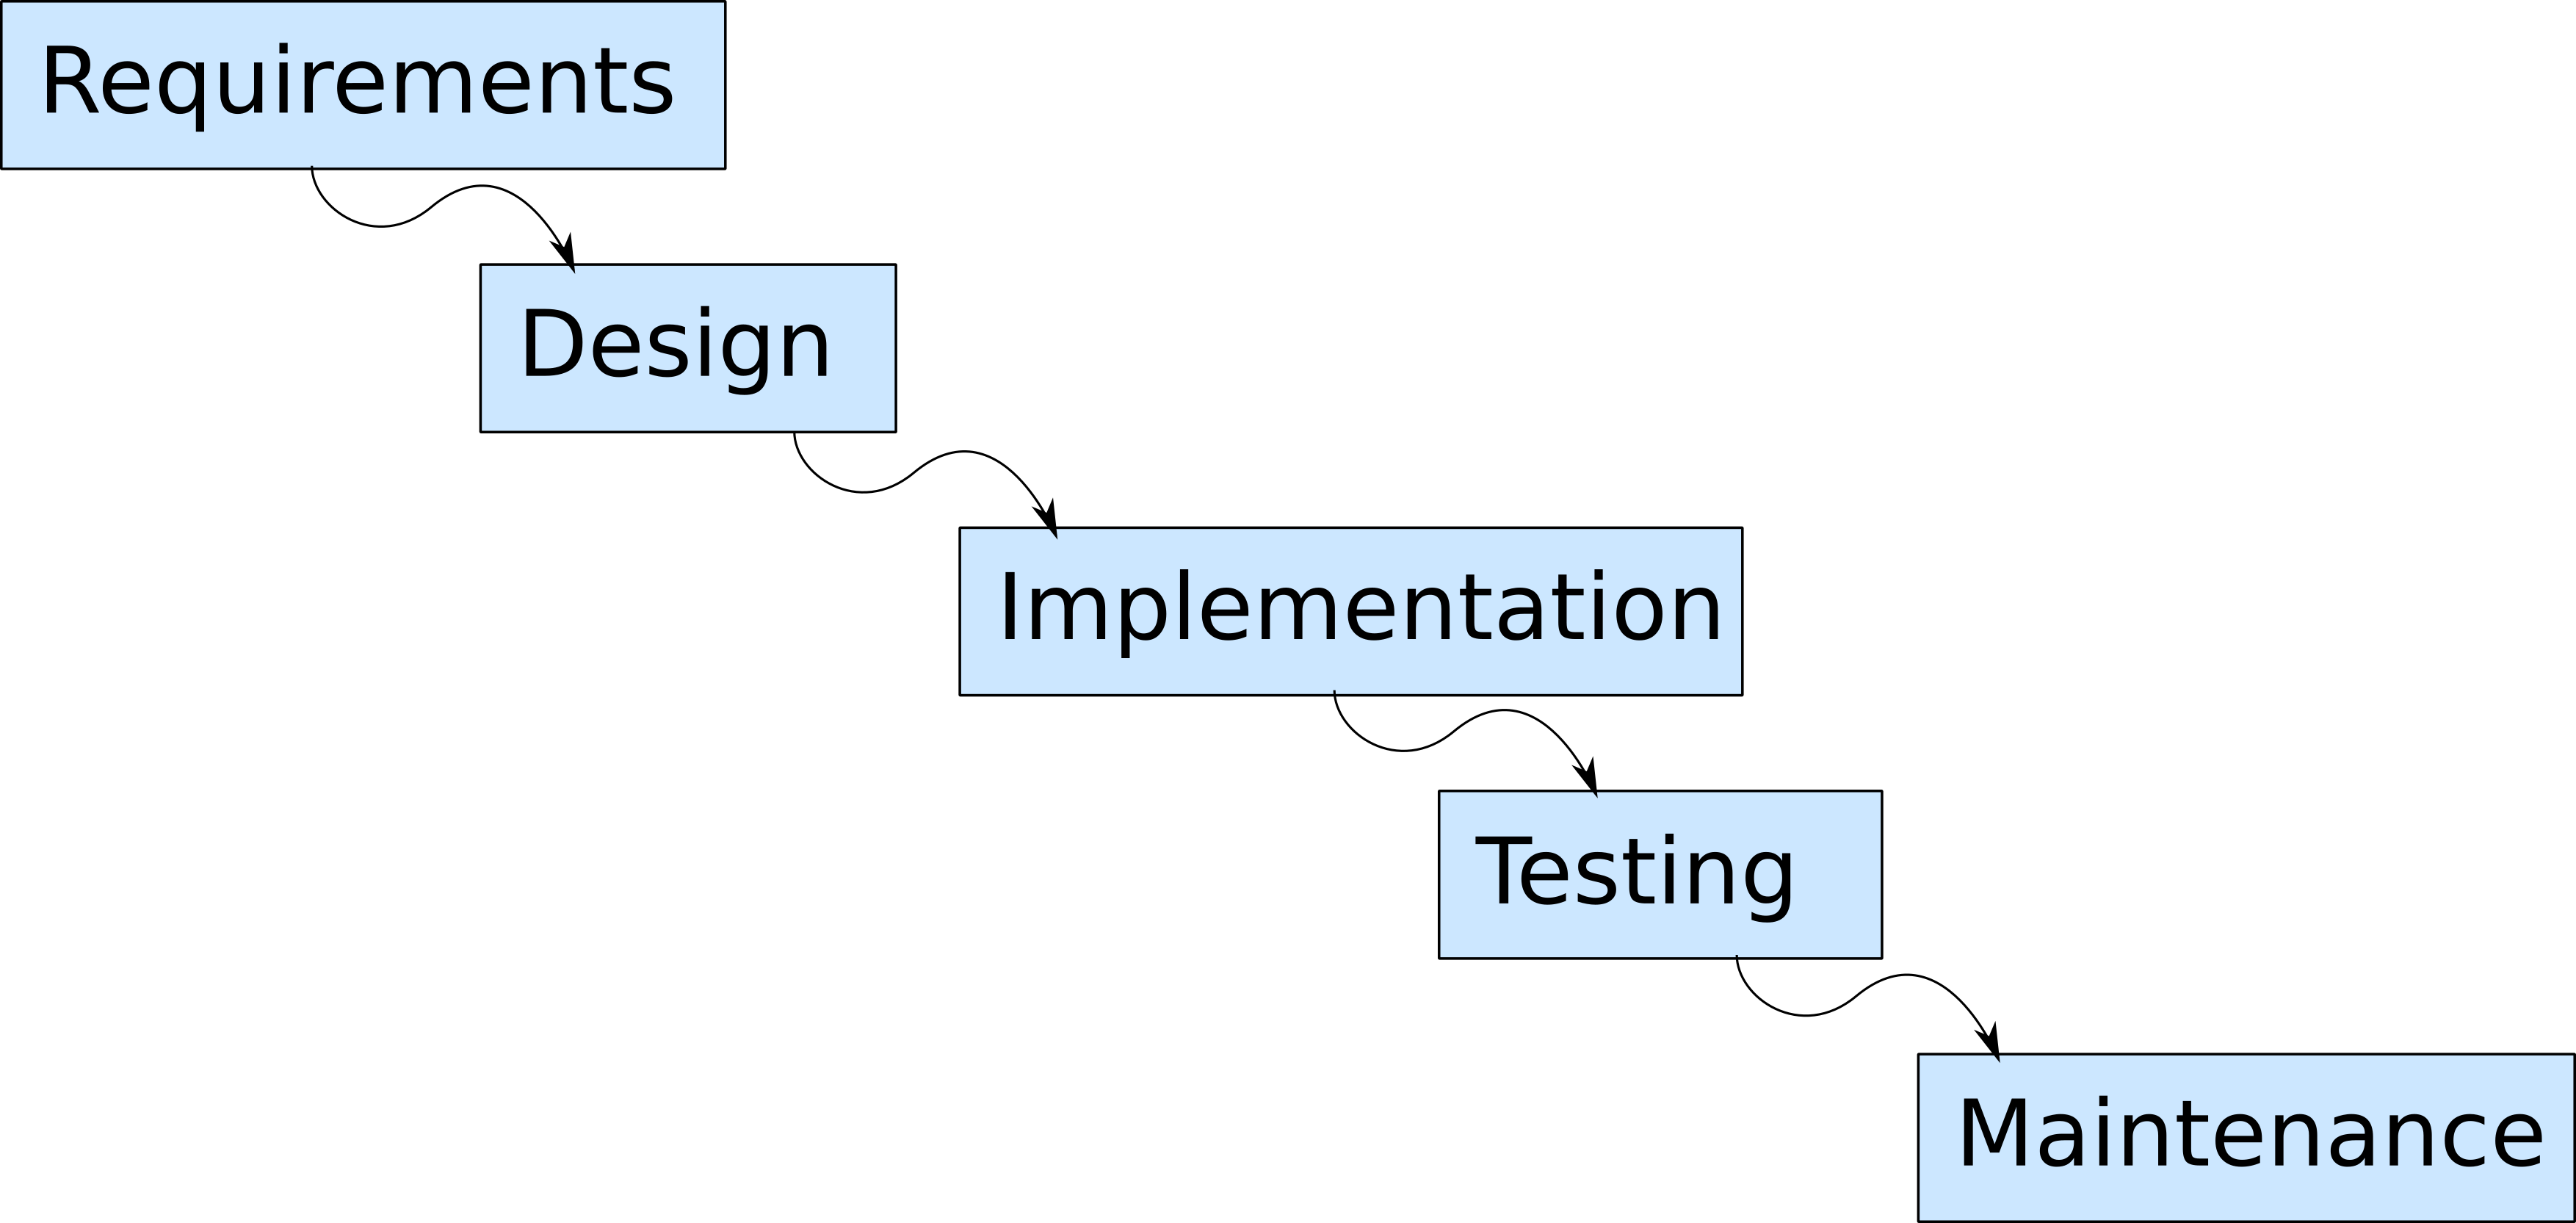
\includegraphics[height=.8\textheight]{safetygfx/waterfall.png}
  
  \note{
  \begin{itemize}
  \item Adapted from civil engineering; dates back to the 1950s
  \item Each phase follows the next; required big-upfront-everything design
  \item Difficult to make changes in later development phases
  \item Clear phase separation is not realistic in practice
  \item Testing happens last and is first to be cut short
  \item Errors are detected late (in testing) and difficult to fix
  \end{itemize}
  }
\end{frame}

\begin{frame}
  \frametitle{The V-Model of Systems Develoment}
  
  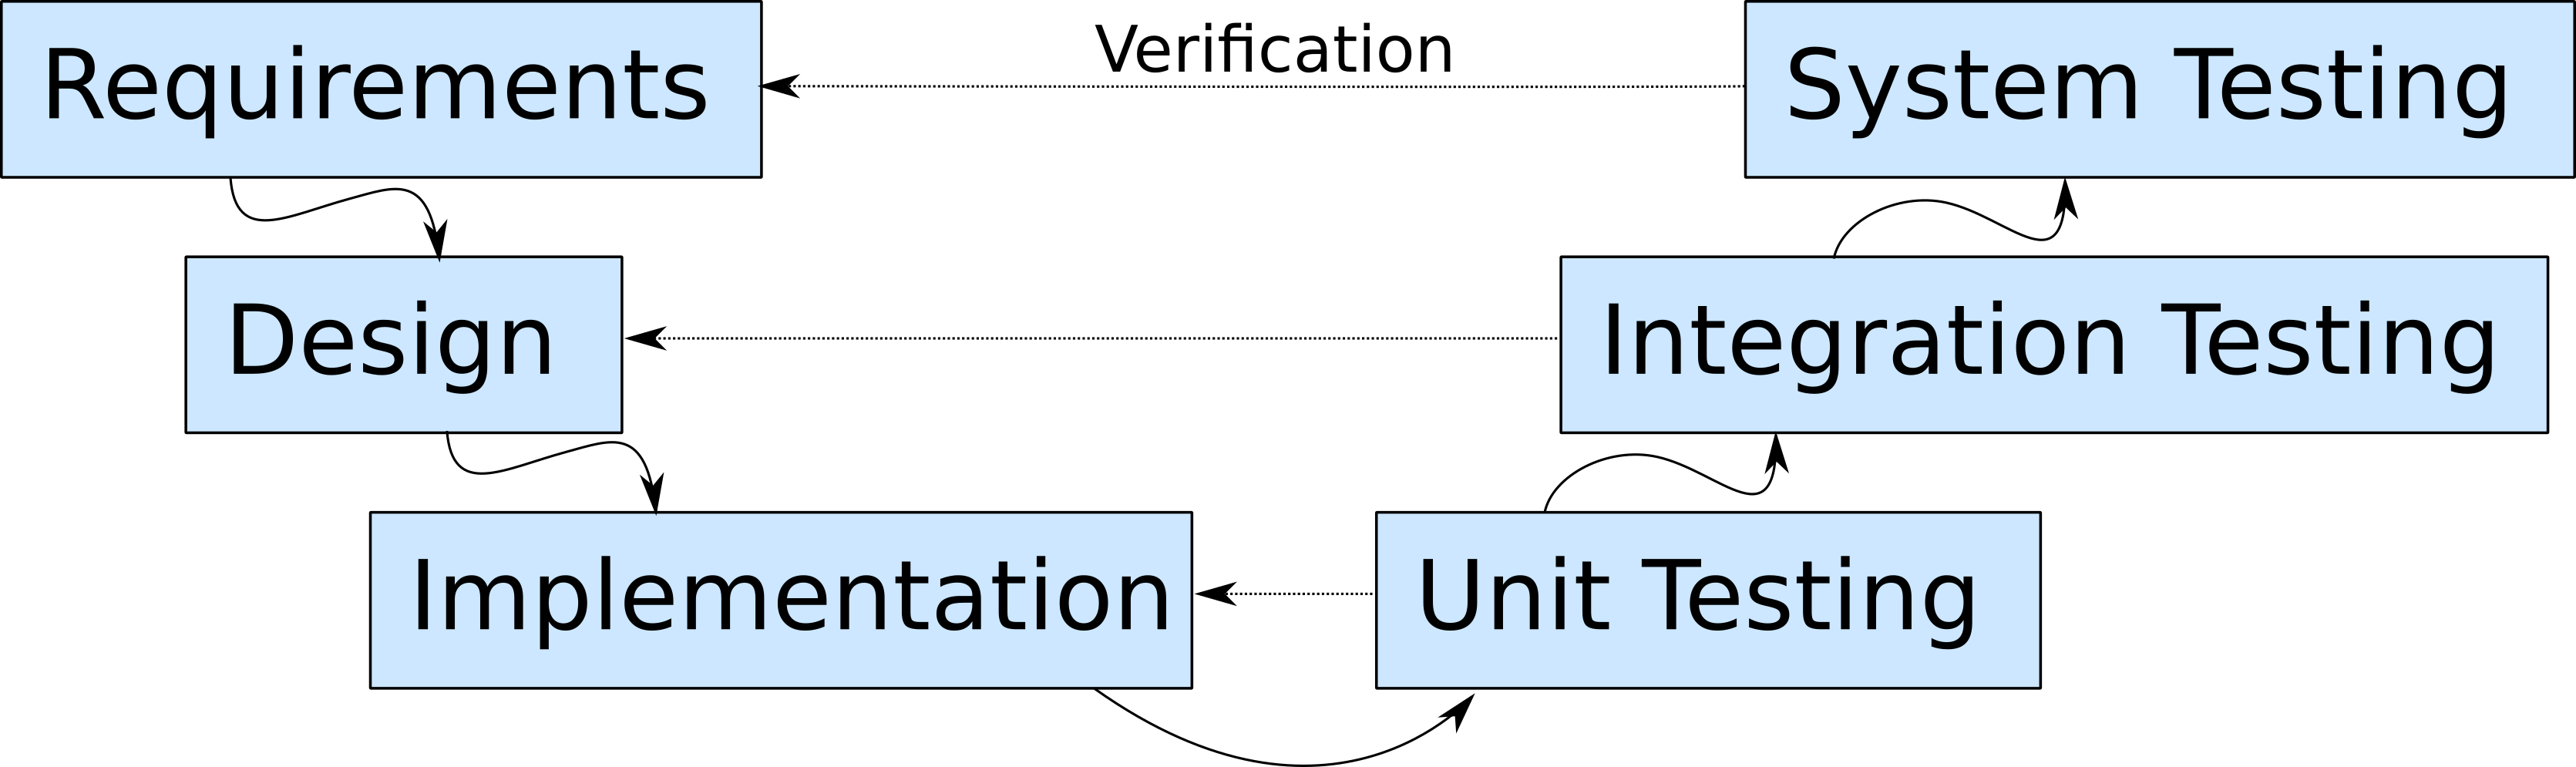
\includegraphics[height=.57\textheight]{safetygfx/v_model.png}
  
  \note{
  \begin{itemize}
  \item Dates back to 1980s; different flavors exist - German V-model for military projects in 1986; civil versions in 1990s
  \item Each testing phase validates the development phase; Agile versions allow relaxing of phases;
  \item Standardized in various versions; basis for most standards for safety critical development; W-model extension
  \end{itemize}
  }
\end{frame}

\begin{frame}
  \frametitle{Product Life Cycle in ISO 26262}
  
  \begin{itemize}
  \item Based on V-model; V of Vs:
  \begin{itemize}
    \item Overall system design
    \item Hardware development 
    \item Software development
  \end{itemize} \cpause
  \item Hazard analysis to identify safety goals   \cpause
  \item Functional safety concept at system level   \cpause
  \item Technical safety concept as input to hardware and software development phases   \cpause
  \item Gives exact definitions of outputs and objectives for each phase   \cpause
  \item Requires traceability between phases across the entire development
  \end{itemize}
\end{frame}

\begin{frame}
  \frametitle{Hazard Analysis and Risk Assessment}
  
  \begin{itemize}
  \item Identify hazardous events on the level of vehicle functions \cpause
  \item Each hazard will have an associated severity and likelihood \cpause
  \item Severity $\times$ Likelihood $=$ Risk \cpause
  \item Risk $\times$ Controllability $=$ ASIL level \cpause
  \item Safety integrity levels: ASIL A, B, C, D; QM \cpause
  \item Outcome: A list of safety goals with ASIL levels
  \end{itemize}
  
  \note{
  \begin{itemize}
  \item Progression: Hazard $\rightarrow$ Hazardous event $\rightarrow$ ASIL Classification
  \item ASIL QM - Quality Management; Risk of hazard is tolerable, no safety requirements
  \end{itemize}
  }
\end{frame}

\begin{frame}
  \frametitle{Quantifying Risk - Safety Integrity Levels}
  
  \begin{itemize}
  \item ASIL classification determines the degree of rigor required in addressing the safety goal \cpause
  \item Fulfilling a higher integrity level implies suitability for lower ASIL levels \cpause
  \item ASIL is always associated to a specific safety goal; but the resulting measures may be applicable independently (e.g. when writing a software library)
  \end{itemize}
\end{frame}

\begin{frame}
  \frametitle{Functional Safety Concept}
  
  Highest level design phase \cpause
  \begin{itemize}
  \item Derive from the safety goals a list of functional safety requirements \cpause
  \item Requirements inherit ASIL from the safety goal \cpause
  \item A single requirement may be associated with multiple safety goals
  \end{itemize}
  
  \note{
  \begin{itemize}
  \item Two outcomes: Functional safety concept and verification report
  \end{itemize}
  }
\end{frame}

\begin{frame}

  \frametitle{Strategies for Achieving Safety Goals}
  
  \begin{itemize}
    \item Avoid the fault causing a hazard \cpause
    \item Detect the fault and control its impact \cpause
    \item Design the system to be fault-tolerant \cpause
    \begin{itemize}
      \item Timing analysis \cpause
      \item Redundancy \cpause
      \item Diversity
    \end{itemize} \cpause
    \item Increase controllability through driver warnings \cpause
    \item Definition of emergency fallback state
  \end{itemize}
  
  \note{
  \begin{itemize}
  \item Fault control: E.g. Transition to a safe state; functional degradation, user-visible impact
  \item Fault tolerance: E.g. de-bouncing of sensor data; redundant systems
  \item Emergency fallback state: Minimum risk maneuver
  \end{itemize}
  }

\end{frame}

\begin{frame}
  \frametitle{Product Development at System Level - Technical Safety Concept}
  
  First development phase \cpause
  \begin{itemize}
  \item Defines the concrete safety mechanisms that will be responsible for fulfilling the safety requirements \cpause
  \item Technical safety requirements take into account concrete details of the implementation \cpause
  \item Technical safety requirements need to be testable \cpause
  \item Describes functionality of mechanisms including timing and tolerance properties \cpause
  \item Input from the system level into the actual software development process
  \end{itemize}
  
  \note{
  \begin{itemize}
  \item HSI
  \item Integration testing plan
  \end{itemize}
  }
  
\end{frame}

\begin{frame}
  \frametitle{Software Development Lifecycle}
  
  The V inside the V.
  \begin{itemize}
  \item Software safety requirements
  \item Software architectural design
  \item Software unit design and implementation
  \item Unit/Integration/System Testing
  \end{itemize}
  
  \note{
  TIMECHECK 0:40
  }
\end{frame}

\begin{frame}
  \frametitle{Software Safety Requirements}
  
  \begin{itemize}
  \item Derived from the Technical Safety Concept \cpause
  \item Describes how software implements the safety-related functionalities \cpause
  \item Refined Hardware/Software interface \cpause
  \item Optional ASIL decomposition \cpause
  \item Requirements get reviewed extensively  \cpause
  \item Basis for software system tests
  \end{itemize}
  
  \note{
  \begin{itemize}
  \item Safety-related functionality: execution of a nominal function; safe or degraded state (transition and maintain); fault detection; self-test; timing-critical (watchdog)
  \item Outcomes:
  \begin{itemize}
      \item SW Safety Requirements Spec
      \item Refined HSI Spec
      \item SW Verification Report
  \end{itemize}
  \end{itemize}
  }
\end{frame}

\begin{frame}
  \frametitle{Software Architectural Design}
  
  \begin{itemize}
  \item Software Design Phase: System must verifiably fulfill the safety requirements \cpause
  \item Software Architecture breaks the system into smaller components \cpause
  \item Describes static and dynamic interaction in a hierarchical structure \cpause
  \item Architects play a vital role in supporting actual verification and implementation efforts
  \end{itemize}
  
  \note{
  \begin{itemize}
  \item First stage where actual software development concerns arise
  \end{itemize}
  }
\end{frame}


%\fi %!!!!!!!!!!!!!!!!!


\begin{frame}
  \frametitle{Software Architectural Design}
  
  Properties of a good Architecture \cpause
  \begin{itemize}
  \item Primary goal is to avoid systematic faults \cpause
  \item Comprehensible, simple, verifiable \cpause
  \item Breakdown into small self-contained pieces \cpause
  \item Clearly defined responsibilities \cpause
  \item Encapsulation of critical data \cpause
  \item Maintainability
  \end{itemize}
  
  \note{
  \begin{itemize}
    \item Hierarchical structure
    \item Restricted size and complexity of components
    \item Restricted size of interfaces
    \item Cohesion of components
    \item Loose coupling
    \item Scheduling, interrupts
    \item Spatial isolation, management of shared resources (global variables)
  \end{itemize}
  }
\end{frame}

\begin{frame}
  \frametitle{Software Architectural Design}
  
  Architecture Description \cpause
  \begin{itemize}
  \item Write documentation! \cpause
  \item Especially in higher ASIL levels, use semi-formal notation in addition to prose \cpause
  \item Architecture needs to be verifiable
  \begin{itemize}
    \item Integration tests
    \item Simulations on the architecture model
  \end{itemize}
  \end{itemize}
\end{frame}

\begin{frame}
  \frametitle{Software Architectural Design}
  
  Special concerns of safety software architecture \cpause
  \begin{itemize}
  \item Partitioning o software components according to their ASIL level (freedom from interference) \cpause
  \item Analysis of dependent failures \cpause
  \item Analysis to provide evidence for suitability of the design to address safety requirements \cpause
  \item Analysis of resource usage and timing constraints \cpause
  \item Design verification
  \end{itemize}
  
  \note{
  Design Verification:
  \begin{itemize}
  \item Walk-through, inspection
  \item Simulation,  Formal verification
  \item Control and data flow analysis, scheduling analysis
  \end{itemize}
  Outcome:
  \begin{itemize}
  \item SW Architectural Design specification
  \item Safety Analysis report
  \item Dependent failures analysis report
  \item SW Verification report
  \end{itemize}
  }
\end{frame}

\begin{frame}
  \frametitle{Safety Element Out Of Context}

  \begin{itemize}
    \item Software architecture depends on requirements derived from a specific vehicle function
    \item Software systems be developed out of context
    \item All implicit requirements of the software must be documented
    \item Additional burden on the integrator to ensure that the context in which the system is used is appropriate
  \end{itemize}
  
  \note{
  TIMECHECK 0:50
  }
\end{frame}

\begin{frame}
  \frametitle{Software Unit Design and implementation}

 \cpause  
  \begin{itemize}
    \item May be auto generated from architecture design model \cpause
    \item Heavily relies on specification form earlier phases \cpause
    \item Main goal is consistency with those specifications \cpause
    \item Simple, readable, comprehensible \cpause
    \item Robust to errors \cpause
    \item Suitable for modification \cpause
    \item Verifiable
  \end{itemize}
  
  \note{
  TIMECHECK 0:60
  \begin{itemize}
    \item Design principles shall be applied to achieve the properties
  \end{itemize}
  }
\end{frame}

\begin{frame}
  \frametitle{Software Unit Design and implementation}

  \tikz[baseline,inner sep=0]\node[anchor=base](ar100){};
  Design Principles \cpause
  \hspace{.1\textwidth}
  \tikz[baseline,inner sep=0]\node[anchor=base](ar200){};
  \begin{itemize}
    \item Single-entry , single-exit \cpause
    \item No dynamic objects \cpause
    \item No uninitialized variables \cpause
    \item No global variables \cpause
    \item No variables of same name \cpause
    \item No pointers \cpause
    \item No hidden data flow or control flow \cpause
    \item No recursion
  \end{itemize}
  \tikz[baseline,inner sep=0]\node[anchor=base](br100){};
  \hspace{.31\textwidth}
  \tikz[baseline,inner sep=0]\node[anchor=base](br200){};
  
  \pause
  \begin{tikzpicture}[remember picture,overlay]
  \draw[line width=30pt,red] (ar200) -- (br100);
  \draw[line width=30pt,red] ([shift={(-0.5\textwidth,0)}]ar100) -- (br200);
  \end{tikzpicture}
  
  Use coding guidelines!
\end{frame}

\begin{frame}
  \frametitle{Requirements for programming languages}
  
  \cpause
  \begin{itemize}
    \item Unambiguous and comprehensible definition \cpause
    \begin{itemize}
      \item Formal language spec (also needed for tool qualification) \cpause
      \item No undefined behavior \cpause
      \item No footguns
    \end{itemize} \cpause
    \item Support modularity, abstraction and encapsulation \cpause
    \item Support structured programming
  \end{itemize}
  
  Criteria not sufficiently addressed by the language itself shall be covered by coding guidelines.
  
  \note{
  TIMECHECK 0:70
  }
\end{frame}

\begin{frame}
  \frametitle{Coding Guidelines}
  
   \cpause
  \begin{itemize}
    \item Subsetting the language \cpause
    \item Enforcement of low complexity \cpause
    \item Enforcement of strong typing \cpause
    \item Concurrency
  \end{itemize}
\end{frame}

\begin{frame}
  \frametitle{MISRA C++}
  
  \begin{itemize}
    \item Discourage use of dangerous language features
    \item Promote best practices
    \item Avoid undefined behavior
  \end{itemize}
  \cpause
  
  \vspace{10pt}
  The guidelines are just one part, the process for enforcing them is just as important.
  \cpause
  
  \vspace{15pt}
  Following guidelines does not guarantee absence of bugs.
  
  \note{
  \begin{itemize}
  \item Dangerous here can also mean non-deterministic runtime
  \item Quality Metrics
  \end{itemize}
  }
\end{frame}

\begin{frame}
  \frametitle{Ensuring Quality - Testing and Verification}
  
   \cpause
  \begin{itemize}
    \item Pair programming and Code reviews \cpause
    \item Static and dynamic code analysis \cpause
    \item (Semi-)Formal verification \cpause
    \item Requirements-based testing \cpause
    \item Fault injection tests \cpause
    \item Resource monitoring
  \end{itemize}
  
  \note{
  TIMECHECK 0:80
  }
\end{frame}

\begin{frame}
  \frametitle{Ensuring Quality - Testing and Verification}
  
  Testing methodologies \cpause
  \begin{itemize}
    \item Analysis of boundary conditions \cpause
    \item Analysis of equivalence classes \cpause
    \item Analysis of functional dependencies \cpause
    \item Coverage metrics \cpause
    \item Testing on actual target hardware \cpause
  \end{itemize}
  
  Testing efforts are continuously monitored and summarized in approved verification reports before production.
\end{frame}

\begin{frame}
  \frametitle{Why do we do all this?}
  
   \cpause
  
  \begin{center}
    Because it works.
  \end{center}
\end{frame}

\begin{frame}
  \frametitle{Conclusion}
  
  \begin{itemize}
    \item Safety is much more than just the programming language
    \item Lots of processes and practices
    \item Most work products from the development are not software
    \item Software development best practices are the same
    \item Creation of an environment that ensures those practices are actually followed
  \end{itemize}
\end{frame}

\begin{frame}
  \frametitle{Thanks for your attention.}

  \href{https://stackoverflow.com/users/577603/comicsansms}{
\includegraphics[height=.05\textheight]{resources/so-icon.png}}
  \href{https://github.com/ComicSansMS}{
\includegraphics[height=.05\textheight]{resources/github-icon.png}}
  \includegraphics[height=.05\textheight]{resources/discord-icon.png} ComicSansMS
  %\includegraphics[height=.05\textheight]{resources/discord-icon.png} ComicSansMS /
  %\href{https://twitter.com/DerGhulbus/}{
\includegraphics[height=.05\textheight]{resources/twitter-icon.png} @DerGhulbus}
  
  \vspace{15pt}
  \href{https://ghulbus-inc.de/}{https://ghulbus-inc.de/}

\end{frame}


\end{document}
